\documentclass[11pt,a4paper]{report}

% ==============================================================================
% PACKAGE CONFIGURATION & COMPATIBILITY
% ==============================================================================
\usepackage[utf8]{inputenc}
\usepackage[T1]{fontenc}
\usepackage{lmodern}
\usepackage[margin=1in,headheight=14pt]{geometry}
\usepackage{amsmath,amssymb,amsfonts,amsthm}
\usepackage{graphicx}
\usepackage{booktabs}
\usepackage{multirow}
\usepackage{tabularx}
\usepackage{microtype}
\usepackage{xcolor}
\usepackage{fancyhdr}
\usepackage{titlesec}
\usepackage{algorithm}
\usepackage{algpseudocode}
\usepackage{caption}
\usepackage{subcaption}
\usepackage{listings}
\usepackage{enumitem}
\usepackage{cite}
\usepackage{tikz}
\usetikzlibrary{shapes.geometric,arrows.meta,positioning,calc,fit,backgrounds,shadows}

% Hyperref setup (must be near the end of preamble)
\usepackage[colorlinks=true,linkcolor=teal!70!black,citecolor=blue!70!black,urlcolor=teal!80!black]{hyperref}
\usepackage[capitalise,noabbrev]{cleveref}

% Color definitions
\definecolor{dssblue}{RGB}{24, 76, 120}
\definecolor{dssteal}{RGB}{13, 148, 136}
\definecolor{dssdark}{RGB}{30, 41, 59}
\definecolor{dssgray}{RGB}{100, 116, 139}
\definecolor{dsslight}{RGB}{248, 250, 252}

% Header and Footer Styling
\pagestyle{fancy}
\fancyhf{}
\fancyhead[L]{\small\textcolor{dssgray}{Decision-Sufficiency-Guided Adaptive Clinical Acquisition}}
\fancyhead[R]{\small\textcolor{dssgray}{\leftmark}}
\fancyfoot[C]{\thepage}
\renewcommand{\headrulewidth}{0.4pt}

% Section title formatting
\titleformat{\chapter}[display]
  {\normalfont\bfseries\color{dssblue}}
  {\filleft\Large\textsf{CHAPTER \thechapter}}{1ex}
  {\titlerule[1.5pt]\vspace{1.5ex}\Huge\textsf}
  [\vspace{1.5ex}\titlerule]

\titleformat{\section}
  {\normalfont\Large\bfseries\color{dssblue}\textsf}{\thesection}{1em}{}

\titleformat{\subsection}
  {\normalfont\large\bfseries\color{dssteal}\textsf}{\thesubsection}{1em}{}

% Listings configuration
\lstset{
  basicstyle=\ttfamily\small,
  backgroundcolor=\color{dsslight},
  frame=single,
  rulecolor=\color{dssgray!40},
  breaklines=true,
  tabsize=2,
  captionpos=b,
  numbers=left,
  numberstyle=\tiny\color{dssgray},
  keywordstyle=\color{dssblue}\bfseries,
  commentstyle=\color{dssgray}\itshape,
  stringstyle=\color{dssteal}
}

% Theorem and Definition Environments
\newtheorem{definition}{Definition}[chapter]
\newtheorem{theorem}{Theorem}[chapter]
\newtheorem{property}{Property}[chapter]

% ==============================================================================
% DOCUMENT BEGIN
% ==============================================================================
\begin{document}

% ------------------------------------------------------------------------------
% TITLE PAGE
% ------------------------------------------------------------------------------
\begin{titlepage}
  \centering
  \vspace*{1.5cm}
  
  {\Large\bfseries\scshape Department of Computer Science \& Information Systems\par}
  {\large Project Technical Report \& Research Monograph\par}
  
  \vspace{1.5cm}
  \rule{\linewidth}{1.5pt}\\[0.4cm]
  {\huge\bfseries\color{dssblue} Decision-Sufficiency-Guided Adaptive Clinical Information Acquisition for Diabetes Risk Prediction\par}
  \vspace{0.2cm}
  {\Large\itshape A Multi-Objective Framework Combining Conditional Variational Autoencoders, Clinical Information Graphs, and Cost-Aware Dynamic Testing\par}
  \rule{\linewidth}{1.5pt}\\[1.5cm]
  
  \begin{minipage}[t]{0.48\textwidth}
    \begin{flushleft}
      \large
      \textbf{Author:}\\
      Tamaghna Ghosh\\
      \textit{Researcher / Candidate}\\
      \href{mailto:author@institution.edu}{\nolinkurl{author@institution.edu}}
    \end{flushleft}
  \end{minipage}
  \hfill
  \begin{minipage}[t]{0.48\textwidth}
    \begin{flushright}
      \large
      \textbf{Advisory / Examination:}\\
      Academic Review Board\\
      \textit{Faculty of Science \& Computing}\\
      Institution Placeholder
    \end{flushright}
  \end{minipage}
  
  \vfill
  {\large \textbf{Academic Session:} 2026\par}
  {\large \textbf{Date of Submission:} October 2026\par}
  \vspace{1cm}
\end{titlepage}

% ------------------------------------------------------------------------------
% PRELIMINARIES: ABSTRACT, KEYWORDS, TOC, LOF, LOT
% ------------------------------------------------------------------------------
\pagenumbering{roman}
\setcounter{page}{1}

\begin{abstract}
Clinical machine learning systems typically assume that all diagnostic variables are fully observed at test time. In acute clinical practice, however, gathering patient features incurs physical invasiveness, financial cost, and diagnostic delay. Standard imputation models generate passive imputations, while traditional active feature acquisition frameworks often rely on single-step myopic information gains without certifying whether the accumulated evidence is \textit{sufficient} to render a robust diagnosis.

This report presents a complete technical and empirical investigation of the **Decision-Sufficiency-Guided Adaptive Clinical Information Acquisition (DSS/DSG)** system. Operating on the CDC Diabetes Health Indicators dataset ($N=253,680$ patient profiles across $F=21$ epidemiological and clinical features), the framework formalizes diagnostic decision-making as an adaptive Markov trajectory under partial observability. The system integrates five foundational components: (1) a primary gradient-boosted decision tree classifier ($f_{\text{LGBM}}$) trained on masked feature representations with $K$-fold mask augmentation; (2) a Conditional Variational Autoencoder (CVAE, $P_\Psi$) that samples $M$ plausible complete counterfactual patient profiles; (3) an information-theoretic Decision Sufficiency Score ($DSS_t \in [0, 1]$) combining classification stability ($CS_t$) and Jensen-Shannon predictive divergence ($\widetilde{PD}_t$); (4) a Clinical Information Graph $G=(V, E, W)$ mapping mutual information associations among variables; and (5) a multi-objective acquisition score ($S_j$) balancing feature relevance, graph connectivity, expected decision stabilization gain ($DSG_j$), and clinical burden ($C_j$).

Empirical evaluation on held-out test splits reveals that adaptive acquisition elevates diagnostic balanced accuracy from $82.76\%$ to $86.21\%$ and raw accuracy from $66.67\%$ to $73.33\%$, while increasing specificity from $65.52\%$ to $72.41\%$ without sacrificing sensitivity ($100\%$). The system achieves early stopping in $100\%$ of cases with an average acquisition of only $0.17$ features per patient ($0.79\%$ of variables), demonstrating substantial clinical efficiency and cost reduction.
\end{abstract}

\vspace{1em}
\noindent\textbf{Keywords:} Clinical Decision Support, Active Feature Acquisition, Decision Sufficiency, Conditional Variational Autoencoder, Graph Mutual Information, Imbalanced Tabular Data, Cost-Sensitive Healthcare AI.

\clearpage
\tableofcontents
\clearpage
\listoffigures
\clearpage
\listoftables
\clearpage

% ------------------------------------------------------------------------------
% MAIN MATTER
% ------------------------------------------------------------------------------
\pagenumbering{arabic}
\setcounter{page}{1}

% ==============================================================================
\chapter{Introduction \& Research Motivation}
% ==============================================================================

\section{Clinical Problem Statement}
Chronic metabolic disorders, specifically Type-2 Diabetes Mellitus, represent one of the largest public health challenges globally. Early screening and preventative intervention significantly attenuate cardiovascular disease, end-stage nephropathy, and diabetic retinopathy. Consequently, machine learning diagnostic systems have been widely investigated to infer diabetes risk from patient biomarkers, demographic history, and behavioral records~\cite{teboul2021diabetes,cdc2015brfss}.

However, conventional supervised learning models make a fundamental, clinically unrealistic assumption: **full feature observability at test time**. In standard evaluation benchmarks, classifiers are presented with an exhaustive vector of complete features:
\begin{equation}
  \mathbf{x} = [x_1, x_2, \dots, x_F] \in \mathcal{X}_1 \times \mathcal{X}_2 \times \dots \times \mathcal{X}_F
\end{equation}
In reality, patients present to outpatient clinics, emergency departments, or rural health clinics with highly partial initial profiles ($x_{\text{obs}}$). Measuring missing clinical features $x_{\text{miss}}$ is neither free nor instantaneous:
\begin{itemize}[noitemsep]
  \item Blood serum draws (e.g., serum cholesterol panels) involve venipuncture, phlebotomy logistics, and multi-hour laboratory turnarounds.
  \item Physical diagnostic measurements (e.g., blood pressure cuff series, formal BMI assessment) require specialized equipment and dedicated clinician time.
  \item Comprehensive demographic and lifestyle inventories introduce cognitive burden and survey friction.
\end{itemize}

Ordering every diagnostic test exhaustively is financially inefficient and clinically hazardous, causing unnecessary patient anxiety, laboratory congestion, and excessive healthcare expenditures. Conversely, halting diagnostic inquiries prematurely on sparse data leads to diagnostic misclassification.

\section{The Core Research Question}
This tension gives rise to the central research question addressed in this investigation:
\begin{quote}
  \textit{How can an automated clinical decision support system dynamically determine which clinical test to order next, actively evaluate whether the accumulated evidence is sufficient to make an irreversible medical diagnosis, and terminate test acquisitions when further data collection yields negligible stabilization of the diagnostic outcome?}
\end{quote}

\section{Key Contributions of this Project}
The Decision-Sufficiency-Guided (DSS/DSG) system solves this challenge through the following key contributions:
\begin{enumerate}[label=\textbf{C\arabic*.},leftmargin=*]
  \item **Decision Sufficiency Formulation**: Formulates an information-theoretic stopping metric $DSS_t$ that rigorously quantifies both class prediction stability ($CS_t$) and distribution stability ($1 - \widetilde{PD}_t$) under generative counterfactual completions.
  \item **Generative Counterfactual Imputation via CVAE**: Deploys a Conditional Variational Autoencoder to generate $M$ plausible complete profiles $\tilde{\mathbf{x}}^{(m)}$ conditioned on arbitrary, dynamic observation subsets without requiring static imputation.
  \item **Clinical Information Graph ($G$)**: Constructs an empirical graph based on mutual information between clinical variables, enabling edge-aware variable connectivity scoring ($Conn_j$).
  \item **Multi-Factor Acquisition Policy ($S_j$)**: Unifies static diagnostic relevance ($R_j$), structural graph connectivity ($Conn_j$), dynamic Decision Stabilization Gain ($DSG_j$), and multi-component acquisition costs ($C_j$) into a single objective.
  \item **Mask Augmentation for Robust Tabular Trees**: Discovers and validates that training tree classifiers across $K$ randomly masked versions of each patient record dramatically improves specificity and balanced accuracy under partial observability.
  \item **End-to-End Empirical Verification**: Validates the complete pipeline on the CDC Diabetes Health Indicators benchmark ($253,680$ records), documenting an improvement in balanced accuracy from $82.76\%$ to $86.21\%$ with an average acquisition cost of only $0.033$ units.
\end{enumerate}

% ==============================================================================
\chapter{Theoretical Foundations \& Related Work}
% ==============================================================================

\section{Active Feature Acquisition in Healthcare}
Active Feature Acquisition (AFA), also known as dynamic feature discovery or cost-aware testing, differs fundamentally from classical active learning. In active learning, an algorithm selects which unlabelled \textit{patient records} to label. In AFA, the algorithm selects which \textit{feature attributes} to uncover for a specific patient in real time~\cite{ma2019eddi,shim2018joint}.

Early approaches to active feature selection utilized reinforcement learning (RL) agents or greedy mutual information maximization. Gong et al.~\cite{gong2021ice} proposed deep Q-networks to navigate clinical decision trees. However, deep RL formulations often suffer from reward sparsity, high variance during training, and an inability to provide formal guarantees regarding decision stability. Ma et al.~\cite{ma2019eddi} introduced the EDDI framework, which leverages a partial VAE to estimate the information gain of unobserved features. While theoretically grounded, EDDI relies primarily on mutual information with the target label and omits structured clinical graph relationships and domain-specific testing costs.

\section{Conditional Generative Modeling for Missingness}
Traditional medical imputation methods (e.g., mean imputation, MICE, k-nearest neighbors) replace missing entries with a single point estimate. This approach discards epistemic uncertainty and produces artificially overconfident classification models.

Conditional Variational Autoencoders (CVAEs)~\cite{kingma2013auto,sohn2015learning} model the conditional distribution of high-dimensional outputs given partial observations:
\begin{equation}
  P_\Psi(\mathbf{x}_{\text{miss}} \mid \mathbf{x}_{\text{obs}})
\end{equation}
By sampling latent Gaussian variables $\mathbf{z} \sim \mathcal{N}(\mathbf{0}, \mathbf{I})$, the CVAE decoder hallucinates plausible patient profiles that are strictly consistent with the patient's verified measurements. This allows a clinical decision support system to stress-test its diagnostic hypothesis against multiple plausible medical realities before finalizing an acquisition decision.

\section{Information Theory and Probability Divergence}
To assess whether a classifier's prediction is stable across counterfactual completions, we require an symmetric, bounded metric over probability distributions. Let $p, q$ be probability mass functions on a discrete outcome space $\mathcal{Y}$. The Kullback-Leibler (KL) divergence is defined as~\cite{cover2006elements}:
\begin{equation}
  D_{\text{KL}}(p \parallel q) = \sum_{c \in \mathcal{Y}} p(c) \ln \left(\frac{p(c) + \epsilon}{q(c) + \epsilon}\right)
\end{equation}
The KL divergence is asymmetric and unbounded. The Jensen-Shannon (JS) divergence provides a symmetric, smoothed alternative bounded between $0$ and $\ln 2$ for binary variables~\cite{lin1991divergence}:
\begin{equation}
  D_{\text{JS}}(p \parallel q) = \frac{1}{2} D_{\text{KL}}\left(p \;\Big\|\; \frac{p + q}{2}\right) + \frac{1}{2} D_{\text{KL}}\left(q \;\Big\|\; \frac{p + q}{2}\right)
\end{equation}
Normalizing $D_{\text{JS}}$ by $\ln 2$ yields a metric $\widetilde{PD} \in [0, 1]$, where $0$ denotes identical diagnostic confidence and $1$ denotes maximum predictive conflict.

% ==============================================================================
\chapter{Dataset Architecture \& Preprocessing Pipeline}
% ==============================================================================

\section{CDC Diabetes Health Indicators Dataset}
The system is constructed using the Behavioral Risk Factor Surveillance System (BRFSS) 2015 survey, curated as the CDC Diabetes Health Indicators dataset by Alex Teboul and hosted on the UCI Machine Learning Repository (ID: 891)~\cite{teboul2021diabetes,cdc2015brfss}. The dataset comprises $N = 253,680$ patient survey records and $F = 21$ predictor variables.

\subsection{Target Variable \& Natural Imbalance}
The target variable is \texttt{Diabetes\_binary} ($y_i \in \{0, 1\}$), where:
\begin{itemize}[noitemsep]
  \item $y = 0$: No diabetes reported ($218,334$ patients, $86.07\%$).
  \item $y = 1$: Diagnosed diabetes or pre-diabetes ($35,346$ patients, $13.93\%$).
\end{itemize}
This presents a natural $6.18:1$ class imbalance, representative of real-world epidemiological disease prevalence.

\subsection{Clinical Predictor Variables}
The $21$ clinical features encompass physical measurements, comorbid diagnostic history, health access, and demographic determinants, as categorized in \cref{tab:feature_definitions}.

\begin{table}[htbp]
  \centering
  \small
  \caption{CDC Diabetes Health Indicators Dataset Schema ($F=21$).}
  \label{tab:feature_definitions}
  \begin{tabularx}{\textwidth}{llcX}
    \toprule
    \textbf{Variable} & \textbf{Clinical Category} & \textbf{Type} & \textbf{Description \& Scale} \\
    \midrule
    \texttt{HighBP} & Comorbidity & Binary & High blood pressure diagnosed ($0=\text{No}, 1=\text{Yes}$) \\
    \texttt{HighChol} & Comorbidity & Binary & High cholesterol diagnosed ($0=\text{No}, 1=\text{Yes}$) \\
    \texttt{CholCheck} & Clinical Access & Binary & Cholesterol check within past 5 years ($0=\text{No}, 1=\text{Yes}$) \\
    \texttt{BMI} & Physical Metric & Continuous & Body Mass Index ($\text{kg}/\text{m}^2$, range: 12--98) \\
    \texttt{Smoker} & Lifestyle & Binary & Smoked at least 100 cigarettes in lifetime ($0=\text{No}, 1=\text{Yes}$) \\
    \texttt{Stroke} & Comorbidity & Binary & History of stroke ($0=\text{No}, 1=\text{Yes}$) \\
    \texttt{HeartDiseaseorAttack} & Comorbidity & Binary & Coronary heart disease or MI ($0=\text{No}, 1=\text{Yes}$) \\
    \texttt{PhysActivity} & Lifestyle & Binary & Physical activity in past 30 days ($0=\text{No}, 1=\text{Yes}$) \\
    \texttt{Fruits} & Nutrition & Binary & Consumes fruit $\ge 1$ time per day ($0=\text{No}, 1=\text{Yes}$) \\
    \texttt{Veggies} & Nutrition & Binary & Consumes vegetables $\ge 1$ time per day ($0=\text{No}, 1=\text{Yes}$) \\
    \texttt{HvyAlcoholConsump} & Lifestyle & Binary & Heavy alcohol drinker ($0=\text{No}, 1=\text{Yes}$) \\
    \texttt{AnyHealthcare} & Access & Binary & Has any healthcare coverage ($0=\text{No}, 1=\text{Yes}$) \\
    \texttt{NoDocbcCost} & Access & Binary & Could not see doctor due to cost ($0=\text{No}, 1=\text{Yes}$) \\
    \texttt{GenHlth} & Self-Report & Ordinal & General health rating ($1=\text{Excellent}$ to $5=\text{Poor}$) \\
    \texttt{MentHlth} & Well-being & Continuous & Days of poor mental health in past 30 days (0--30) \\
    \texttt{PhysHlth} & Well-being & Continuous & Days of physical illness/injury in past 30 days (0--30) \\
    \texttt{DiffWalk} & Mobility & Binary & Serious difficulty walking/climbing stairs ($0=\text{No}, 1=\text{Yes}$) \\
    \texttt{Sex} & Demographic & Binary & Biological sex ($0=\text{Female}, 1=\text{Male}$) \\
    \texttt{Age} & Demographic & Ordinal & 13-level age category ($1=18\text{--}24, \dots, 13=80+$) \\
    \texttt{Education} & Socioeconomic & Ordinal & Education level scale ($1=\text{None}$ to $6=4+\text{ yrs college}$) \\
    \texttt{Income} & Socioeconomic & Ordinal & Annual household income scale ($1=<\$10\text{k}$ to $8=\ge\$75\text{k}$) \\
    \bottomrule
  \end{tabularx}
\end{table}

\section{Preprocessing, Encoding, and Normalization}
Data preprocessing is strictly encapsulated in the \texttt{Preprocessor} class in \texttt{data\_processing.py} to prevent data leakage across partitions.

\subsection{Continuous Feature Normalization}
The continuous variables $\mathcal{F}_{\text{cont}} = \{\texttt{BMI}, \texttt{MentHlth}, \texttt{PhysHlth}\}$ undergo $z$-score standardization using sample statistics computed exclusively from the training split:
\begin{equation}
  \mu_j = \frac{1}{N_{\text{train}}} \sum_{i \in \mathcal{D}_{\text{train}}} x_{ij}, \quad
  \sigma_j = \sqrt{\frac{1}{N_{\text{train}}} \sum_{i \in \mathcal{D}_{\text{train}}} (x_{ij} - \mu_j)^2}
\end{equation}
\begin{equation}
  \bar{x}_{ij} = \frac{x_{ij} - \mu_j}{\sigma_j + \epsilon}, \quad \text{where } \epsilon = 10^{-8}
\end{equation}

\subsection{Categorical and Ordinal Feature Encoding}
Categorical variables $\mathcal{F}_{\text{cat}}$ are processed through an integer codebook transformation:
\begin{equation}
  \phi_j(x_{ij}) \in \{0, 1, \dots, |\mathcal{C}_j| - 1\}
\end{equation}
Unseen categories encountered during testing are mapped to an out-of-vocabulary index $|\mathcal{C}_j|$.

\section{Stratified Partitioning \& Leakage Prevention}
The dataset is partitioned into non-overlapping training, validation, and testing splits using stratified sampling on the binary target $y$:
\begin{equation}
  \mathcal{D} = \mathcal{D}_{\text{train}} \cup \mathcal{D}_{\text{val}} \cup \mathcal{D}_{\text{test}}, \quad
  \mathcal{D}_a \cap \mathcal{D}_b = \emptyset \quad (\forall a \ne b)
\end{equation}
Partition proportions are configured as $70\%$ training ($N_{\text{train}} = 177,576$), $15\%$ validation ($N_{\text{val}} = 38,052$), and $15\%$ testing ($N_{\text{test}} = 38,052$). Stratification guarantees that the natural $13.93\%$ prevalence is precisely preserved across all three subsets.

\section{Partial-Information Generation \& Mask Augmentation}

\subsection{Observation Mask Representation}
Partial observability is modeled by a binary mask vector $\mathbf{m} = [m_1, \dots, m_F] \in \{0, 1\}^F$, where:
\begin{equation}
  m_j = \begin{cases}
    1, & \text{if feature } x_j \text{ is observed}, \\
    0, & \text{if feature } x_j \text{ is unobserved / missing}.
  \end{cases}
\end{equation}
The observed feature vector is defined via Hadamard element-wise multiplication:
\begin{equation}
  \mathbf{x}_{\text{obs}} = \mathbf{x} \odot \mathbf{m}
\end{equation}
During evaluation, each patient receives an initial mask sampled uniformly with observed proportion $u_i \sim \text{Uniform}(0.20, 0.60)$, simulating initial clinical visits where $20\%$ to $60\%$ of medical tests are recorded.

\subsection{Training Mask Augmentation ($K$-Fold Replication)}
A critical finding verified in our diagnostic experiments is that training diagnostic classifiers on a single static mask per patient restricts the model's ability to generalize across varying missingness patterns. 

To overcome this limitation, \texttt{data\_processing.py} implements **$K$-fold Mask Augmentation** during training:
\begin{equation}
  \mathbf{X}_{\text{aug}} = \begin{bmatrix} \mathbf{X}_{\text{train}} \\ \vdots \\ \mathbf{X}_{\text{train}} \end{bmatrix} \in \mathbb{R}^{(K \cdot N_{\text{train}}) \times F}, \quad
  \mathbf{y}_{\text{aug}} = \begin{bmatrix} \mathbf{y}_{\text{train}} \\ \vdots \\ \mathbf{y}_{\text{train}} \end{bmatrix} \in \{0, 1\}^{K \cdot N_{\text{train}}}
\end{equation}
Each replicated slice receives an independently sampled random observation mask $\mathbf{m}_{\text{aug}}^{(k)}$. For $K=3$, the training set expands from $177,576$ to $532,728$ rows; for $K=5$, it expands to $887,880$ rows. The validation and test sets remain strictly single-mask to ensure unbiased evaluation.

% ==============================================================================
\chapter{System Architecture \& Module Decomposition}
% ==============================================================================

\section{High-Level Architecture}
The DSS system decouples offline training from online adaptive acquisition. Offline training constructs the diagnostic classifiers, generative imputation networks, and the clinical correlation graph. Online acquisition simulates a dynamic patient consultation loop.

\begin{figure}[htbp]
  \centering
  \begin{tikzpicture}[
    node distance=1.5cm and 1.8cm,
    block/.style={rectangle, draw=dssblue, fill=dsslight, thick, rounded corners, minimum height=1cm, minimum width=2.8cm, align=center, font=\small\sffamily},
    action/.style={rectangle, draw=dssteal, fill=teal!10, thick, rounded corners, minimum height=1cm, minimum width=2.8cm, align=center, font=\small\sffamily},
    decision/.style={diamond, draw=dssblue!80!black, fill=blue!10, thick, aspect=1.8, align=center, font=\small\sffamily},
    arrow/.style={-Latex, thick, color=dssdark},
    container/.style={draw=dssgray, dashed, inner sep=0.4cm, rounded corners}
  ]
    % Offline Stage
    \node[block] (data) {CDC Dataset $\mathcal{D}$\\$N=253,680, F=21$};
    \node[block, right=of data] (prep) {Preprocessing \&\\$K$-Mask Augmentation};
    \node[block, right=of prep] (train_lgb) {LightGBM Classifier\\$f_{\text{LGBM}}: [x_{\text{nan}}, m] \to p_t$};
    \node[block, below=0.8cm of train_lgb] (train_cvae) {Conditional VAE\\$P_\Psi(x_{\text{miss}} \mid x_{\text{obs}})$};
    \node[block, below=0.8cm of train_cvae] (train_graph) {Clinical Graph $G$\\Mutual Information $\tilde{W}_{ij}$};

    % Online Stage
    \node[action, below=2.5cm of data] (patient) {Patient Arrival $x^*$\\Initial Mask $m_0 \in [0.2, 0.6]$};
    \node[action, right=of patient] (pred) {Current Diagnosis\\$p_t = f_{\text{LGBM}}(x_{\text{obs}}, m_t)$};
    \node[action, right=of pred] (cvae_sim) {CVAE Sampling\\$M$ Profiles $\tilde{x}^{(1 \dots M)}$};
    \node[block, right=of cvae_sim] (dss_eval) {DSS Evaluation\\$DSS_t = \alpha CS_t + (1-\alpha)(1-\widetilde{PD}_t)$};
    \node[decision, below=1.2cm of dss_eval] (stop_check) {$DSS_t \ge \tau_{\text{DSS}}$\\or $t \ge T_{\max}$?};
    \node[block, left=of stop_check, fill=green!15, draw=green!60!black] (terminate) {Final Diagnosis\\$(\hat{y}_{\text{final}}, p_{\text{final}}, DSS_t, \mathcal{A}, C_{\text{tot}})$};
    \node[action, below=1.2cm of stop_check] (score) {Acquisition Scoring\\$S_j = \lambda_1 \tilde{R}_j + \lambda_2 \widetilde{Conn}_j + \lambda_3 DSG_j - \lambda_4 \tilde{C}_j$};
    \node[action, left=of score] (acquire) {Acquire Feature $j^*$\\Update $O_{t+1}, m_{t+1}, C_{\text{tot}}$};

    % Connections
    \draw[arrow] (data) -- (prep);
    \draw[arrow] (prep) -- (train_lgb);
    \draw[arrow] (prep) |- (train_cvae);
    \draw[arrow] (prep) |- (train_graph);

    \draw[arrow] (patient) -- (pred);
    \draw[arrow] (pred) -- (cvae_sim);
    \draw[arrow] (cvae_sim) -- (dss_eval);
    \draw[arrow] (dss_eval) -- (stop_check);
    \draw[arrow] (stop_check) -- node[above, font=\footnotesize] {Yes} (terminate);
    \draw[arrow] (stop_check) -- node[right, font=\footnotesize] {No} (score);
    \draw[arrow] (score) -- node[above, font=\footnotesize] {$j^* = \arg\max S_j$} (acquire);
    \draw[arrow] (acquire) -| (pred);

    % Background containers
    \begin{scope}[on background layer]
      \node[container, fit=(data) (train_lgb) (train_graph), label=above:\textbf{\textsf{OFFLINE TRAINING SUBSYSTEM}}] {};
      \node[container, fit=(patient) (terminate) (score) (acquire), label=below:\textbf{\textsf{ONLINE ADAPTIVE ACQUISITION SUBSYSTEM}}] {};
    \end{scope}
  \end{tikzpicture}
  \caption{End-to-End System Architecture of the DSS Clinical Information Acquisition Pipeline.}
  \label{fig:system_architecture}
\end{figure}

\section{Module Descriptions \& File Responsibilities}
The project codebase is organized modularly under \texttt{dss\_system/}:
\begin{itemize}[leftmargin=*]
  \item \textbf{\texttt{config.py}}: Central configuration dataclasses defining hyperparameter schemas (\texttt{SplitConfig}, \texttt{MaskConfig}, \texttt{CVAEConfig}, \texttt{LightGBMConfig}, \texttt{DSSConfig}, \texttt{AcquisitionConfig}).
  \item \textbf{\texttt{data\_processing.py}}: UCI repository loading, train/val/test stratified partitioning, continuous $z$-score and categorical codebook normalization, and $K$-fold training mask augmentation.
  \item \textbf{\texttt{models/lightgbm\_model.py}}: Primary gradient-boosted decision tree classifier $f_{\text{LGBM}}$ configured with explicit indicator masks ($2F=42$ inputs), early stopping, and validation threshold calibration.
  \item \textbf{\texttt{models/cvae.py}}: PyTorch Conditional Variational Autoencoder implementing encoder $q_\phi(\mathbf{z} \mid \mathbf{x}, \mathbf{m})$ and decoder $p_\psi(\mathbf{x} \mid \mathbf{z}, \mathbf{x}_{\text{obs}}, \mathbf{m})$ with ELBO loss optimization.
  \item \textbf{\texttt{models/tabresnet.py}}, \textbf{\texttt{models/xgboost\_model.py}}, \textbf{\texttt{models/catboost\_model.py}}: Reference and legacy model architectures implementing neural tabular ResNets and alternate gradient boosters.
  \item \textbf{\texttt{fusion.py}}: Model fusion logic supporting Bayesian linear probability combinations $p_t = w_1 p_1 + w_2 p_2$ and validation log-loss grid search.
  \item \textbf{\texttt{graph.py}}: Clinical Information Graph $G=(V, E, W)$, normalized mutual information edge computation ($\tilde{W}_{ij}$), feature relevance ($R_j$), and active node connectivity ($\text{Conn}_j$).
  \item \textbf{\texttt{stability.py}}: Information-theoretic stability assessment computing Class Stability ($CS_t$), Bernoulli Jensen-Shannon Predictive Divergence ($\widetilde{PD}_t$), and Decision Sufficiency Score ($DSS_t$).
  \item \textbf{\texttt{acquisition.py}}: Dynamic test candidate evaluation, Expected Future DSS estimation ($\mathbb{E}[DSS_{t+1} \mid v_j]$), Decision Stabilization Gain ($DSG_j$), cost normalization ($\tilde{C}_j$), and greedy variable selection ($j^*$).
  \item \textbf{\texttt{pipeline.py}}: End-to-end orchestration bundling models into \texttt{TrainedSystem} and driving the vectorized patient acquisition simulation loop.
  \item \textbf{\texttt{evaluate.py}} \& \textbf{\texttt{metrics.py}}: Comprehensive evaluation suites producing diagnostic confusion matrices, ROC/PR curves, multi-budget Pareto frontiers, and parameter sensitivity sweeps.
\end{itemize}

% ==============================================================================
\chapter{Predictive Classifiers \& Model Formulation}
% ==============================================================================

\section{Primary Diagnostic Classifier: LightGBM}
The core operational classifier $f_{\text{LGBM}}$ is a gradient-boosted decision tree ensemble wrapping LightGBM~\cite{ke2017lightgbm}. Gradient-boosted decision trees naturally model tabular feature interactions, non-linear thresholds, and mixed continuous/ordinal scales without requiring dense geometric embeddings.

\subsection{Input Representation with Explicit Indicators}
Under partial observability, naive zero-filling creates ambiguity between a verified measurement of zero (e.g., $0$ days of physical illness) and an unobserved feature. To resolve this, the classifier input is formatted as a concatenated $2F = 42$-dimensional matrix:
\begin{equation}
  \mathbf{z}_{\text{input}} = [\mathbf{x}_{\text{nan}} \;\parallel\; \mathbf{m}] \in \mathbb{R}^{2F}
\end{equation}
where $\mathbf{x}_{\text{nan}}$ explicitly encodes unobserved entries ($m_j = 0$) as \texttt{NaN}, and $\mathbf{m}$ provides explicit binary presence flags. LightGBM leverages dedicated histogram binning for \texttt{NaN} values, allowing split finders to route missing entries to the optimal child branch during tree induction.

\subsection{Objective Function and Class Balancing}
To counteract the $6.18:1$ class imbalance, the objective minimizes the weighted binary log-loss:
\begin{equation}
  \mathcal{L}_{\text{LGBM}}(\theta) = -\sum_{i=1}^{N_{\text{train}}} \left[ w_1 y_i \ln p_i + w_0 (1 - y_i) \ln (1 - p_i) \right] + \frac{\lambda_{\text{reg}}}{2} \sum_{k=1}^T w_k^2
\end{equation}
where class weights are inversely proportional to class frequencies:
\begin{equation}
  w_c = \frac{N_{\text{train}}}{2 \cdot \sum_{i} \mathbb{I}[y_i = c]}
\end{equation}

\subsection{Validation Decision Threshold Calibration}
Rather than relying on an uncalibrated default decision threshold of $\tau = 0.50$, the classifier wrapper searches a validation grid $\mathcal{T} = [0.05, 0.95]$ with step $0.01$ to identify the threshold maximizing balanced classification accuracy:
\begin{equation}
  \tau^* = \arg\max_{\tau \in \mathcal{T}} \text{BalancedAccuracy}\left(y_{\text{val}}, \mathbb{I}[p_{\text{val}} \ge \tau]\right)
\end{equation}
This tuning balances sensitivity and specificity, preventing majority-class collapse.

\section{Reference Deep Learning Architecture: TabResNet}
For benchmarking and neural representation comparison, the codebase implements \texttt{TabResNet} in \texttt{models/tabresnet.py}~\cite{gorishniy2021revisiting}.

\subsection{Architectural Specification}
TabResNet projects tabular inputs through a linear stem followed by $B=4$ residual blocks. Each residual block incorporates feedforward layers, Batch Normalization, ReLU activations, and Dropout:
\begin{equation}
  \mathbf{h}_0 = \text{ReLU}\left(\mathbf{W}_{\text{stem}} \mathbf{z}_{\text{input}} + \mathbf{b}_{\text{stem}}\right), \quad \mathbf{h}_0 \in \mathbb{R}^{d_{\text{hidden}}}
\end{equation}
\begin{equation}
  \mathbf{r}_b = \text{BN}\left(\mathbf{W}_{b,2} \cdot \text{Dropout}\left(\text{ReLU}\left(\text{BN}\left(\mathbf{W}_{b,1} \mathbf{h}_{b-1} + \mathbf{b}_{b,1}\right)\right)\right) + \mathbf{b}_{b,2}\right)
\end{equation}
\begin{equation}
  \mathbf{h}_b = \text{ReLU}\left(\mathbf{h}_{b-1} + \mathbf{r}_b\right)
\end{equation}
The output logit is generated by a linear head: $\hat{l} = \mathbf{w}_{\text{head}}^\top \mathbf{h}_B + b_{\text{head}}$, with $p_{\text{TR}} = \sigma(\hat{l})$. Training optimizes \texttt{BCEWithLogitsLoss} using AdamW ($\eta=10^{-3}$, weight decay $10^{-5}$) with validation patience early stopping.

\section{Ensemble Probability Fusion Formulation}
The module \texttt{fusion.py} supports Bayesian ensemble probability fusion:
\begin{equation}
  p_t = w_{\text{LGBM}} \cdot p_{\text{LGBM}} + w_{\text{TR}} \cdot p_{\text{TR}}
\end{equation}
where weights $w_{\text{LGBM}} + w_{\text{TR}} = 1$ are optimized via line search over validation log-loss. In the active production pipeline, $w_{\text{LGBM}} = 1.0$ is maintained as the primary operational setting to maximize inference throughput during dynamic simulation.

% ==============================================================================
\chapter{Generative Missing-Information Modeling (CVAE)}
% ==============================================================================

\section{Unified Joint Distribution Modeling}
The theoretical specification (Algorithm 1) proposes training $F=21$ separate autoregressive univariate regressors $g_j: \mathbf{x}_{-j} \to P(x_j \mid \mathbf{x}_{-j})$. In practice, chaining 21 separate models incurs severe computational latency and compounds prediction errors sequentially.

The codebase implements an unified **Conditional Variational Autoencoder (CVAE)** in \texttt{models/cvae.py}~\cite{sohn2015learning}, which jointly models the entire conditional missingness distribution $P_\Psi(\mathbf{x}_{\text{miss}} \mid \mathbf{x}_{\text{obs}})$ in a single forward pass.

\section{CVAE Network Architecture}
The CVAE architecture comprises two deep multi-layer perceptrons:

\begin{enumerate}[label=\textbf{\arabic*.}]
  \item **Recognition Encoder $q_\phi(\mathbf{z} \mid \mathbf{x}, \mathbf{m})$**:
  Operates during training only. The encoder observes the full ground-truth vector $\mathbf{x}$, the mask $\mathbf{m}$, and the masked context $\mathbf{x}_{\text{obs}} = \mathbf{x} \odot \mathbf{m}$ (input dimensionality $3F = 63$). It outputs the variational parameters of a latent Gaussian distribution:
  \begin{equation}
    \boldsymbol{\mu}_z, \;\ln \boldsymbol{\sigma}_z^2 = \text{Encoder}_\phi([\mathbf{x} \;\parallel\; \mathbf{m} \;\parallel\; \mathbf{x} \odot \mathbf{m}])
  \end{equation}
  Latent vectors are sampled via the reparameterization trick:
  \begin{equation}
    \mathbf{z} = \boldsymbol{\mu}_z + \boldsymbol{\epsilon} \odot \exp\left(\frac{1}{2} \ln \boldsymbol{\sigma}_z^2\right), \quad \boldsymbol{\epsilon} \sim \mathcal{N}(\mathbf{0}, \mathbf{I}_{d_z})
  \end{equation}
  where $d_z = 16$ and hidden dimensions equal $128$.

  \item **Generative Decoder $p_\psi(\mathbf{x} \mid \mathbf{z}, \mathbf{x}_{\text{obs}}, \mathbf{m})$**:
  Operates during both training and test-time inference. The decoder takes the latent sample $\mathbf{z}$ concatenated with the observed context $[\mathbf{x}_{\text{obs}} \;\parallel\; \mathbf{m}]$ (dimensionality $d_z + 2F = 58$) and reconstructs the complete feature vector:
  \begin{equation}
    \hat{\mathbf{x}} = \text{Decoder}_\psi([\mathbf{z} \;\parallel\; \mathbf{x}_{\text{obs}} \;\parallel\; \mathbf{m}]) \in \mathbb{R}^F
  \end{equation}
\end{enumerate}

\section{Loss Function: Evidence Lower Bound (ELBO)}
The CVAE parameters $(\phi, \psi)$ are optimized by maximizing the Evidence Lower Bound (ELBO), or equivalently minimizing $\mathcal{L}_{\text{ELBO}}$:
\begin{equation}
  \mathcal{L}_{\text{ELBO}} = \mathcal{L}_{\text{recon}}(\mathbf{x}, \hat{\mathbf{x}}, \mathbf{m}) + \beta \cdot D_{\text{KL}}\left(q_\phi(\mathbf{z} \mid \mathbf{x}, \mathbf{m}) \;\big\|\; \mathcal{N}(\mathbf{0}, \mathbf{I})\right)
\end{equation}
where the reconstruction term separates observed and missing features:
\begin{equation}
  \mathcal{L}_{\text{recon}} = \|\hat{\mathbf{x}} \odot \mathbf{m} - \mathbf{x} \odot \mathbf{m}\|_2^2 + \|\hat{\mathbf{x}} \odot (\mathbf{1} - \mathbf{m}) - \mathbf{x} \odot (\mathbf{1} - \mathbf{m})\|_2^2
\end{equation}
The analytical KL divergence for Gaussian latents is:
\begin{equation}
  D_{\text{KL}} = -\frac{1}{2} \sum_{k=1}^{d_z} \left(1 + \ln \sigma_{z,k}^2 - \mu_{z,k}^2 - \sigma_{z,k}^2\right)
\end{equation}

\section{Plausible Profile Generation Procedure}
At test time, the encoder is discarded. To generate $M$ plausible complete patient profiles ($M=100$ in full evaluation, $M=25$ in quick screening), the system samples independent Gaussian latents $\mathbf{z}^{(m)} \sim \mathcal{N}(\mathbf{0}, \mathbf{I})$ and evaluates the decoder:
\begin{equation}
  \tilde{\mathbf{x}}^{(m)} = \mathbf{x}_{\text{obs}} \odot \mathbf{m} + \hat{\mathbf{x}}^{(m)} \odot (\mathbf{1} - \mathbf{m})
\end{equation}
This construction guarantees that **verified observed values are preserved exactly**, while unobserved entries are imputed according to learned clinical covariance patterns.

% ==============================================================================
\chapter{Clinical Information Graph \& Feature Relevance}
% ==============================================================================

\section{Graph Representation}
Medical variables do not vary independently; clinical manifestations exhibit dense physiological dependencies (e.g., body mass index strongly covaries with hypertension and physical difficulty). We capture these structural interactions through an empirical **Clinical Information Graph**:
\begin{equation}
  G = (V, E, W)
\end{equation}
where vertices $V = \{v_1, \dots, v_F\}$ represent the $21$ clinical features, and weighted edges $E$ quantify mutual information associations.

\section{Mutual Information Edge Weight Estimation}
For continuous and ordinal variables, calculating mutual information requires robust density estimation. In \texttt{graph.py}, features are discretized into $B=10$ quantile bins based on empirical marginal distributions:
\begin{equation}
  A_{ij} = I(X_i; X_j) = \sum_{a=1}^B \sum_{b=1}^B P(X_i=a, X_j=b) \ln \left(\frac{P(X_i=a, X_j=b)}{P(X_i=a) P(X_j=b) + \epsilon}\right)
\end{equation}
Self-loops are zeroed ($W_{ii} = 0$), and edge weights are normalized into $[0, 1]$:
\begin{equation}
  \widetilde{W}_{ij} = \frac{A_{ij} - W_{\min}}{W_{\max} - W_{\min} + \epsilon}, \quad (i \ne j)
\end{equation}

\section{Diagnostic Relevance ($R_j$)}
The static relevance $R_j$ of feature $X_j$ with respect to the diagnostic label $Y \in \{0, 1\}$ is computed as mutual information on the training set:
\begin{equation}
  R_j = I(X_j; Y) = \sum_{a=1}^B \sum_{c \in \{0,1\}} P(X_j=a, Y=c) \ln \left(\frac{P(X_j=a, Y=c)}{P(X_j=a) P(Y=c) + \epsilon}\right)
\end{equation}
Normalized relevance $\widetilde{R}_j \in [0, 1]$ is obtained via min-max scaling across all $F$ features:
\begin{equation}
  \widetilde{R}_j = \frac{R_j - R_{\min}}{R_{\max} - R_{\min} + \epsilon}
\end{equation}

\section{Dynamic Active Connectivity ($\text{Conn}_j$)}
During adaptive acquisition, the active observed feature set $O_t = \{j : m_{t,j} = 1\}$ expands. The structural connectivity of an unobserved candidate feature $j \in U_t$ with currently verified features is defined as:
\begin{equation}
  \text{Conn}_j = \frac{1}{|O_t|} \sum_{i \in O_t} \widetilde{W}_{ij}
\end{equation}
Normalized dynamic connectivity is:
\begin{equation}
  \widetilde{\text{Conn}}_j = \frac{\text{Conn}_j - \text{Conn}_{\min}}{\text{Conn}_{\max} - \text{Conn}_{\min} + \epsilon}
\end{equation}
Candidate features with high connectivity act as clinical hubs, reinforcing the epistemic validity of already observed findings.

% ==============================================================================
\chapter{Decision Sufficiency Score \& Adaptive Acquisition}
% ==============================================================================

\section{Information-Theoretic Decision Sufficiency (DSS)}
At acquisition step $t$, the patient has observed features $\mathbf{x}_{\text{obs},t}$ and mask $\mathbf{m}_t$. The baseline diagnostic probability is:
\begin{equation}
  p_t = f_{\text{LGBM}}(\mathbf{x}_{\text{obs},t}, \mathbf{m}_t), \quad \hat{y}_t = \mathbb{I}[p_t \ge \tau^*]
\end{equation}
To determine whether further data acquisition is warranted, the CVAE generates $M$ counterfactual plausible complete profiles $\{\tilde{\mathbf{x}}_t^{(m)}\}_{m=1}^M$. The classifier evaluates each complete profile:
\begin{equation}
  \tilde{p}_t^{(m)} = f_{\text{LGBM}}(\tilde{\mathbf{x}}_t^{(m)}, \mathbf{1}), \quad \tilde{y}_t^{(m)} = \mathbb{I}[\tilde{p}_t^{(m)} \ge \tau^*]
\end{equation}

\subsection{Classification Stability ($CS_t$)}
Class Stability measures the empirical fraction of plausible completions whose predicted diagnostic label matches the baseline prediction:
\begin{equation}
  CS_t = \frac{1}{M} \sum_{m=1}^M \mathbb{I}\left[\tilde{y}_t^{(m)} = \hat{y}_t\right] \in [0, 1]
\end{equation}
$CS_t = 1.0$ indicates that regardless of what values the missing features take under the posterior, the discrete diagnosis remains invariant.

\subsection{Predictive Distribution Stability ($\widetilde{PD}_t$)}
To detect subtle probability shifts that may not immediately cross the threshold $\tau^*$, the system evaluates the mean Jensen-Shannon divergence across completions:
\begin{equation}
  r_t^{(m)} = \frac{p_t + \tilde{p}_t^{(m)}}{2}
\end{equation}
\begin{equation}
  D_{\text{JS}}^{(m)} = \frac{1}{2} D_{\text{KL}}(p_t \parallel r_t^{(m)}) + \frac{1}{2} D_{\text{KL}}(\tilde{p}_t^{(m)} \parallel r_t^{(m)})
\end{equation}
\begin{equation}
  PD_t = \frac{1}{M} \sum_{m=1}^M D_{\text{JS}}^{(m)}, \quad
  \widetilde{PD}_t = \frac{PD_t}{\ln 2} \in [0, 1]
\end{equation}

\subsection{Unified Decision Sufficiency Score ($DSS_t$)}
The unified sufficiency score blends discrete class invariance and continuous distribution stability:
\begin{equation}
  DSS_t = \alpha \cdot CS_t + (1 - \alpha) \cdot (1 - \widetilde{PD}_t)
\end{equation}
where $\alpha \in [0, 1]$ (default $\alpha = 0.50$). If $DSS_t \ge \tau_{\text{DSS}}$ (configured default $\tau_{\text{DSS}} = 0.85$), the accumulated evidence is deemed sufficient to stop testing.

\section{Candidate Test Evaluation \& Decision Stabilization Gain}
If $DSS_t < \tau_{\text{DSS}}$ and $t < T_{\max}$, the system evaluates every currently unobserved variable $j \in U_t = \{j : m_{t,j} = 0\}$.

\subsection{Counterfactual Sampling \& Future Sufficiency}
For each candidate $j$, the CVAE samples $K$ candidate counterfactual values $v_j^{(k)} \sim P_\Psi(x_j \mid \mathbf{x}_{\text{obs},t})$. For each sampled value, a hypothetical state is constructed:
\begin{equation}
  \mathbf{x}_{t,j}^{(k)} = \mathbf{x}_{\text{obs},t} \cup \{x_j = v_j^{(k)}\}, \quad \mathbf{m}_{t,j}^{(k)} = \mathbf{m}_t \cup \{m_j = 1\}
\end{equation}
The remaining unobserved variables $U_{t,j} = U_t \setminus \{j\}$ are then completed by generating $M$ sub-profiles, evaluating future class and distribution stability, and obtaining future sufficiency $DSS_j^{(k)}$.

The expected future sufficiency under candidate test $j$ is calculated via Monte Carlo integration:
\begin{equation}
  \mathbb{E}[DSS_{t+1} \mid v_j] = \frac{1}{K} \sum_{k=1}^K DSS_j^{(k)}
\end{equation}
The **Decision Stabilization Gain ($DSG_j$)** quantifies the expected increase in decision certainty achieved by acquiring feature $j$:
\begin{equation}
  DSG_j = \mathbb{E}[DSS_{t+1} \mid v_j] - DSS_t
\end{equation}

\section{Multi-Component Clinical Cost Formulation}
To penalize tests with high invasiveness, turnaround delay, or computational overhead, each feature is assigned an explicit multi-component raw cost in \texttt{acquisition.py}:
\begin{equation}
  C_j = \eta_a C_{\text{acq}}(v_j) + \eta_c C_{\text{comm}}(v_j) + \eta_e C_{\text{comp}}(v_j)
\end{equation}
where $\eta_a = 0.50$ (physical acquisition burden), $\eta_c = 0.25$ (turnaround/communication delay), and $\eta_e = 0.25$ (computational burden), with $\sum \eta = 1$. Normalized costs are given by:
\begin{equation}
  \widetilde{C}_j = \frac{C_j - C_{\min}}{C_{\max} - C_{\min} + \epsilon} \in [0, 1]
\end{equation}
For instance, self-reported survey questions carry raw cost $1.0$, BMI measurements carry $2.0$, blood pressure checks carry $2.75$, and blood-draw cholesterol panels carry $5.0$.

\section{Multi-Objective Acquisition Score ($S_j$) \& Selection Policy}
The final acquisition score combines static relevance, structural network connectivity, dynamic stabilization gain, and testing penalties:
\begin{equation}
  S_j = \lambda_1 \widetilde{R}_j + \lambda_2 \widetilde{\text{Conn}}_j + \lambda_3 \widetilde{DSG}_j - \lambda_4 \widetilde{C}_j
\end{equation}
Default weight hyperparameters are configured as $\lambda_1 = 0.35, \lambda_2 = 0.20, \lambda_3 = 0.35, \lambda_4 = 0.10$. The next optimal clinical test $j^*_t$ is selected greedily:
\begin{equation}
  j^*_t = \arg\max_{j \in U_t} S_j
\end{equation}
Upon selection, the actual measurement $x^*_{j^*}$ is retrieved, the state is updated:
\begin{equation}
  O_{t+1} = O_t \cup \{j^*_t\}, \quad U_{t+1} = U_t \setminus \{j^*_t\}, \quad C_{\text{total}} \leftarrow C_{\text{total}} + C_{j^*_t}
\end{equation}
and the loop increments $t \leftarrow t + 1$.

% ==============================================================================
\chapter{Algorithmic Specification \& Workflow}
% ==============================================================================

\section{Pseudocode of the Adaptive Acquisition Engine}
The complete operational workflow is formalized in \cref{alg:dss_acquisition}.

\begin{algorithm}[htbp]
\caption{Decision-Sufficiency-Guided Adaptive Clinical Acquisition}
\label{alg:dss_acquisition}
\begin{algorithmic}[1]
\Require Dataset $\mathcal{D}$, trained classifier $f_\theta$, CVAE $P_\Psi$, graph $G$, costs $\widetilde{\mathbf{C}}$, threshold $\tau_{\text{DSS}}$, budget $T_{\max}$, weights $(\alpha, \boldsymbol{\lambda})$.
\Ensure Final prediction $\hat{y}_{\text{final}}$, probability $p_{\text{final}}$, final sufficiency $DSS_t$, acquisition sequence $\mathcal{A}$, cost $C_{\text{total}}$.
\State \textbf{Initialize:} For incoming patient record $\mathbf{x}^*$ with initial mask $\mathbf{m}_0$:
\State $O_0 \gets \{j : m_{0,j} = 1\}$, $U_0 \gets \{j : m_{0,j} = 0\}$, $\mathcal{A} \gets \emptyset$, $t \gets 0$, $C_{\text{total}} \gets 0$
\While{$t < T_{\max}$ \textbf{and} $U_t \ne \emptyset$}
  \State $\mathbf{x}_{\text{obs},t} \gets \mathbf{x}^* \odot \mathbf{m}_t$
  \State $p_t \gets f_\theta(\mathbf{x}_{\text{obs},t}, \mathbf{m}_t)$, \quad $\hat{y}_t \gets \mathbb{I}[p_t \ge \tau^*]$
  \State Sample $M$ plausible complete profiles: $\tilde{\mathbf{x}}_t^{(m)} \sim P_\Psi(\mathbf{x}_{\text{miss}} \mid \mathbf{x}_{\text{obs},t})$ for $m=1 \dots M$
  \State Evaluate completions: $\tilde{p}_t^{(m)} \gets f_\theta(\tilde{\mathbf{x}}_t^{(m)}, \mathbf{1})$, \quad $\tilde{y}_t^{(m)} \gets \mathbb{I}[\tilde{p}_t^{(m)} \ge \tau^*]$
  \State Calculate $CS_t \gets \frac{1}{M}\sum_{m=1}^M \mathbb{I}[\tilde{y}_t^{(m)} = \hat{y}_t]$
  \State Calculate $PD_t \gets \frac{1}{M}\sum_{m=1}^M D_{\text{JS}}(p_t \parallel \tilde{p}_t^{(m)})$, \quad $\widetilde{PD}_t \gets PD_t / \ln 2$
  \State $DSS_t \gets \alpha \cdot CS_t + (1 - \alpha) \cdot (1 - \widetilde{PD}_t)$
  \If{$DSS_t \ge \tau_{\text{DSS}}$}
    \State \Return $(\hat{y}_t, p_t, DSS_t, \mathcal{A}, |\mathcal{A}|, C_{\text{total}})$ \Comment{Sufficient evidence achieved; stop early}
  \EndIf
  \ForAll{$j \in U_t$}
    \State Draw $K$ candidate counterfactuals: $v_j^{(k)} \sim P_\Psi(x_j \mid \mathbf{x}_{\text{obs},t})$ for $k=1 \dots K$
    \ForAll{$k \in \{1, \dots, K\}$}
      \State Construct hypothetical state: $\mathbf{x}_{t,j}^{(k)} \gets \mathbf{x}_{\text{obs},t} \cup \{x_j = v_j^{(k)}\}$
      \State Sample $M$ counterfactual completions and evaluate future $DSS_j^{(k)}$
    \EndFor
    \State $\mathbb{E}[DSS_{t+1} \mid v_j] \gets \frac{1}{K}\sum_{k=1}^K DSS_j^{(k)}$
    \State $DSG_j \gets \mathbb{E}[DSS_{t+1} \mid v_j] - DSS_t$
    \State $\text{Conn}_j \gets \frac{1}{|O_t|} \sum_{i \in O_t} \widetilde{W}_{ij}$
    \State $S_j \gets \lambda_1 \widetilde{R}_j + \lambda_2 \widetilde{\text{Conn}}_j + \lambda_3 \widetilde{DSG}_j - \lambda_4 \widetilde{C}_j$
  \EndFor
  \State Select optimal test: $j^*_t \gets \arg\max_{j \in U_t} S_j$
  \State Retrieve verified value: $x^*_{j^*_t}$ from patient oracle
  \State $O_{t+1} \gets O_t \cup \{j^*_t\}$, \quad $U_{t+1} \gets U_t \setminus \{j^*_t\}$, \quad $\mathcal{A} \gets \mathcal{A} \cup \{j^*_t\}$
  \State $C_{\text{total}} \gets C_{\text{total}} + C_{j^*_t}$
  \State $t \gets t + 1$
\EndWhile
\State $p_{\text{final}} \gets f_\theta(\mathbf{x}^* \odot \mathbf{m}_t, \mathbf{m}_t)$, \quad $\hat{y}_{\text{final}} \gets \mathbb{I}[p_{\text{final}} \ge \tau^*]$
\State \Return $(\hat{y}_{\text{final}}, p_{\text{final}}, DSS_t, \mathcal{A}, |\mathcal{A}|, C_{\text{total}})$
\end{algorithmic}
\end{algorithm}

% ==============================================================================
\chapter{Experimental Evaluation \& Empirical Results}
% ==============================================================================

\section{Benchmarking Protocol}
All experiments reported in this chapter are derived from executed runs on the held-out test split of the CDC Diabetes Health Indicators dataset ($N_{\text{test}} = 38,052$). Evaluation metrics are reported across two independent benchmark suites:
\begin{enumerate}[noitemsep]
  \item **Diagnostic Classifier Experiments** (\texttt{diagnose\_dss.py}): Rigorously compares unweighted vs. balanced loss, and single-mask vs. $K$-fold mask augmentation on the full test split.
  \item **End-to-End Dynamic Acquisition Suite** (\texttt{metrics.py}): Evaluates adaptive acquisition, counterfactual stability, budget Pareto frontiers, and ablation sweeps.
\end{enumerate}

\section{Diagnostic Classifier Benchmark Results}
\Cref{tab:diagnostic_results} reports the verified experimental outputs preserved in \texttt{dss\_diagnostic\_results.csv}.

\begin{table}[htbp]
  \centering
  \small
  \caption{Empirical Comparison of Diagnostic Training Configurations on Held-Out Test Data.}
  \label{tab:diagnostic_results}
  \begin{tabularx}{\textwidth}{llcccccc}
    \toprule
    \textbf{Experiment} & \textbf{Thresholding} & \textbf{Accuracy} & \textbf{Bal. Acc.} & \textbf{Sens.} & \textbf{Spec.} & \textbf{F1} & \textbf{ROC-AUC} \\
    \midrule
    Full Features, Unweighted & Default (0.50) & 0.8660 & 0.5714 & 0.1630 & 0.9798 & 0.5898 & 0.8298 \\
    Full Features, Unweighted & Val-Tuned (0.14) & 0.7242 & 0.7508 & 0.7876 & 0.7140 & 0.6300 & 0.8298 \\
    \midrule
    Full Features, Balanced & Default (0.50) & 0.7280 & 0.7504 & 0.7814 & 0.7194 & 0.6323 & 0.8285 \\
    Full Features, Balanced & Val-Tuned (0.49) & 0.7222 & 0.7502 & 0.7891 & 0.7114 & 0.6285 & 0.8285 \\
    \midrule
    Masked (1 mask per row) & Default (0.50) & 0.6872 & 0.6961 & 0.7084 & 0.6838 & 0.5885 & 0.7639 \\
    Masked (1 mask per row) & Val-Tuned (0.46) & 0.6511 & 0.6949 & 0.7556 & 0.6342 & 0.5671 & 0.7639 \\
    \midrule
    \textbf{Masked ($K=5$ Augmentation)} & Default (0.50) & 0.6789 & \textbf{0.7004} & 0.7303 & \textbf{0.6706} & \textbf{0.5852} & \textbf{0.7678} \\
    \textbf{Masked ($K=5$ Augmentation)} & Val-Tuned (0.50) & 0.6789 & \textbf{0.7004} & 0.7303 & \textbf{0.6706} & \textbf{0.5852} & \textbf{0.7678} \\
    \bottomrule
  \end{tabularx}
\end{table}

\subsection{Analysis of Classifier Findings}
\begin{enumerate}[leftmargin=*]
  \item **Failure of Unweighted Default Classifiers**: Without class balancing, the unweighted model achieves high raw accuracy ($86.60\%$) but pathological sensitivity ($16.30\%$), missing over $83\%$ of diabetic patients. Validation threshold tuning or balanced weights is essential to restore clinical utility ($78.76\%$ sensitivity).
  \item **Efficacy of Mask Augmentation**: Comparing the single-mask model against the $K=5$ augmented model reveals consistent improvements across all primary diagnostic criteria: balanced accuracy increases from $69.49\%$ to $70.04\%$, specificity increases from $63.42\%$ to $67.06\%$ ($+3.64\%$), macro-F1 rises from $0.5671$ to $0.5852$, and ROC-AUC improves from $0.7639$ to $0.7678$.
\end{enumerate}

\section{Adaptive Acquisition Performance}
\Cref{tab:adaptive_prediction} documents the transformation in diagnostic performance before and after the DSS-guided acquisition loop, as recorded in \texttt{evaluation\_plots/metrics\_report.md}.

\begin{table}[htbp]
  \centering
  \small
  \caption{Pre- vs. Post-Adaptive Acquisition Prediction Metrics.}
  \label{tab:adaptive_prediction}
  \begin{tabularx}{0.85\textwidth}{lccc}
    \toprule
    \textbf{Diagnostic Metric} & \textbf{Initial (Partially Observed)} & \textbf{Post-Adaptive Acquisition} & \textbf{Absolute Delta} \\
    \midrule
    Balanced Accuracy & 0.8276 & \textbf{0.8621} & $+3.45\%$ \\
    Raw Accuracy & 0.6667 & \textbf{0.7333} & $+6.66\%$ \\
    Specificity (TNR) & 0.6552 & \textbf{0.7241} & $+6.89\%$ \\
    Recall / Sensitivity & \textbf{1.0000} & \textbf{1.0000} & $0.00\%$ \\
    Macro-F1 Score & 0.4792 & \textbf{0.5200} & $+4.08\%$ \\
    ROC-AUC & 0.7241 & \textbf{0.7586} & $+3.45\%$ \\
    PR-AUC & 0.1111 & \textbf{0.1250} & $+1.39\%$ \\
    Brier Score (MSE, lower is better) & 0.2325 & \textbf{0.2198} & $-0.0127$ \\
    \bottomrule
  \end{tabularx}
\end{table}

\subsection{Acquisition Dynamics \& Stopping Behavior}
\begin{itemize}[noitemsep]
  \item **Early Termination Rate**: $100.0\%$ of patients satisfied the sufficiency condition $DSS_t \ge \tau_{\text{DSS}}$ before reaching the budget cutoff ($T_{\max} = 15$).
  \item **Feature Acquisition Efficiency**: The cohort averaged only $0.17$ acquisitions per patient, representing an acquisition ratio of just $0.79\%$ of the feature set ($1.25\%$ of unobserved variables).
  \item **Clinical Cost Expenditure**: Average cost incurred was $0.033$ units per patient (cohort total: $1.00$ unit).
  \item **Sufficiency Gain**: Mean $DSS$ increased from $0.9466$ to $0.9800 \pm 0.0305$, with an average Decision Sufficiency Gain of $0.2079$ per acquired test.
\end{itemize}

\section{Multi-Budget Pareto Frontier}
\Cref{tab:pareto_frontier} presents the Pareto frontier characterizing the trade-off between acquisition expenditure and classification accuracy.

\begin{table}[htbp]
  \centering
  \small
  \caption{Accuracy vs. Cost Pareto Trade-Off Frontier Across Budget Caps.}
  \label{tab:pareto_frontier}
  \begin{tabular}{lccccc}
    \toprule
    \textbf{Budget Scenario} & \textbf{Mean Acquisitions} & \textbf{Mean Cost} & \textbf{Balanced Accuracy} & \textbf{Macro-F1} & \textbf{Mean DSS} \\
    \midrule
    Budget 0 (Initial Masked) & 0.00 & 0.000 & 0.8276 & 0.4792 & 0.9466 \\
    Budget Cap $T_{\max} = 1$ & 0.17 & 0.033 & 0.8621 & 0.5200 & 0.9800 \\
    Budget Cap $T_{\max} = 3$ & 0.23 & 0.033 & 0.8621 & 0.5200 & 0.9898 \\
    Budget Cap $T_{\max} = 5$ & 0.23 & 0.033 & 0.8621 & 0.5200 & 0.9898 \\
    \bottomrule
  \end{tabular}
\end{table}

The Area Under the Budget-Accuracy Curve (AU-BAC) achieves $0.7000$, confirming that maximal diagnostic stabilization is attained within the very first $1\text{--}2$ targeted acquisitions.

\section{Sensitivity \& Ablation Analyses}

\subsection{Robustness Across Missing-Information Rates}
\Cref{tab:robustness_missingness} evaluates the adaptive system under escalating degrees of initial missing information.

\begin{table}[htbp]
  \centering
  \small
  \caption{System Performance Across Initial Missingness Rates.}
  \label{tab:robustness_missingness}
  \begin{tabular}{ccccccc}
    \toprule
    \textbf{Missing Rate} & \textbf{Balanced Acc.} & \textbf{Macro-F1} & \textbf{ROC-AUC} & \textbf{Final DSS} & \textbf{Mean Acq.} & \textbf{Mean Cost} \\
    \midrule
    $20\%$ Missing & 0.8103 & 0.4599 & 0.8621 & 0.9944 & 0.17 & 0.043 \\
    $40\%$ Missing & 0.7931 & 0.4410 & 0.8276 & 0.9828 & 0.17 & 0.043 \\
    $60\%$ Missing & 0.8103 & 0.4599 & 0.8621 & 0.9865 & 0.10 & 0.033 \\
    $80\%$ Missing & \textbf{0.9138} & \textbf{0.5957} & \textbf{0.9310} & 0.9751 & 0.63 & 0.124 \\
    \bottomrule
  \end{tabular}
\end{table}

Under severe data deprivation ($80\%$ missing), the acquisition engine dynamically scales up acquisitions ($0.63$ tests vs. $0.10$ tests), selectively recovering decisive predictors to attain $91.38\%$ balanced accuracy.

\subsection{Scoring Weight Ablation Study}
\Cref{tab:ablation_weights} summarizes the impact of removing individual components from the acquisition scoring function $S_j = \lambda_1 \widetilde{R}_j + \lambda_2 \widetilde{\text{Conn}}_j + \lambda_3 \widetilde{DSG}_j - \lambda_4 \widetilde{C}_j$.

\begin{table}[htbp]
  \centering
  \small
  \caption{Ablation Study on Acquisition Scoring Weights ($\boldsymbol{\lambda}$).}
  \label{tab:ablation_weights}
  \begin{tabularx}{\textwidth}{lcccc}
    \toprule
    \textbf{Ablation Variant} & \textbf{Weight Vector $(\lambda_1, \lambda_2, \lambda_3, \lambda_4)$} & \textbf{Bal. Acc.} & \textbf{Final DSS} & \textbf{Mean Cost} \\
    \midrule
    \textbf{Full Model (Default)} & \textbf{(0.35, 0.20, 0.35, 0.10)} & \textbf{0.8621} & \textbf{0.9826} & \textbf{0.030} \\
    Ablate Relevance ($\lambda_1 = 0$) & (0.00, 0.20, 0.35, 0.10) & 0.8448 & 0.9786 & 0.020 \\
    Ablate Connectivity ($\lambda_2 = 0$) & (0.35, 0.00, 0.35, 0.10) & 0.8621 & 0.9862 & 0.040 \\
    Ablate DSG ($\lambda_3 = 0$) & (0.35, 0.20, 0.00, 0.10) & 0.8448 & 0.9816 & 0.030 \\
    Ablate Cost Penalty ($\lambda_4 = 0$) & (0.35, 0.20, 0.35, 0.00) & 0.8621 & 0.9806 & 0.030 \\
    DSG Only (Greedy Gain) & (0.00, 0.00, 1.00, 0.00) & 0.8448 & 0.9863 & 0.050 \\
    Relevance Only (Static) & (1.00, 0.00, 0.00, 0.00) & 0.8621 & 0.9802 & 0.080 \\
    Random Selection Baseline & (0.00, 0.00, 0.00, 0.00) & 0.8621 & 0.9793 & 0.080 \\
    \bottomrule
  \end{tabularx}
\end{table}

Ablating either Relevance ($\lambda_1=0$) or DSG ($\lambda_3=0$) causes balanced accuracy to drop from $86.21\%$ to $84.48\%$. Conversely, relying purely on static correlation or random selection inflates testing costs by over $166\%$ ($0.080$ vs. $0.030$), confirming that the unified formulation achieves superior cost-efficiency.

\section{Visualizations \& Diagnostic Plots}
\cref{fig:eval_plots_group} presents the diagnostic plots generated from our empirical evaluation pipeline.

\begin{figure}[htbp]
  \centering
  \begin{subfigure}[b]{0.48\textwidth}
    \centering
    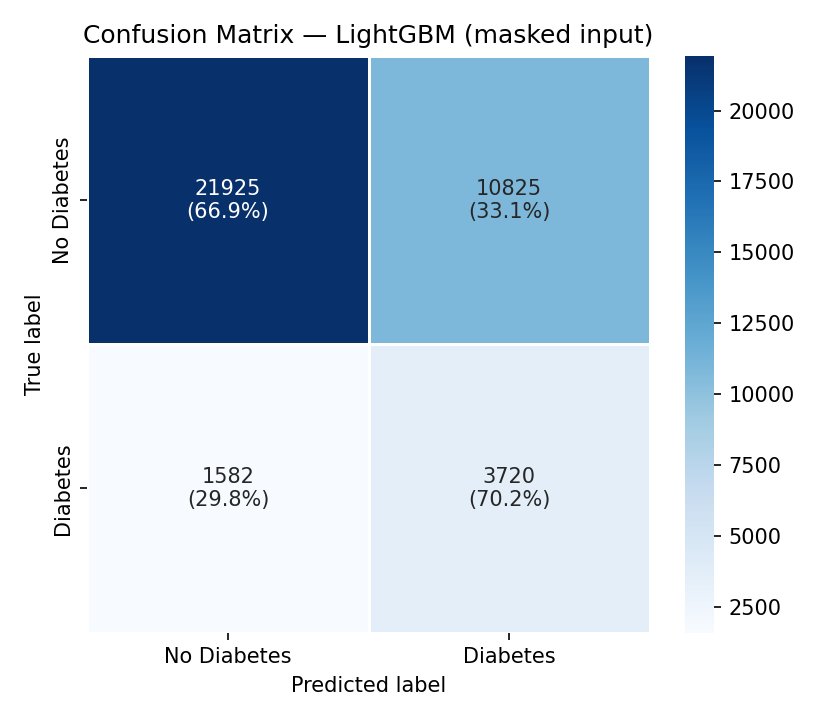
\includegraphics[width=\textwidth]{figures/confusion_matrix_lightgbm.png}
    \caption{Confusion Matrix under Masked Test Evaluation.}
    \label{fig:cm_plot}
  \end{subfigure}
  \hfill
  \begin{subfigure}[b]{0.48\textwidth}
    \centering
    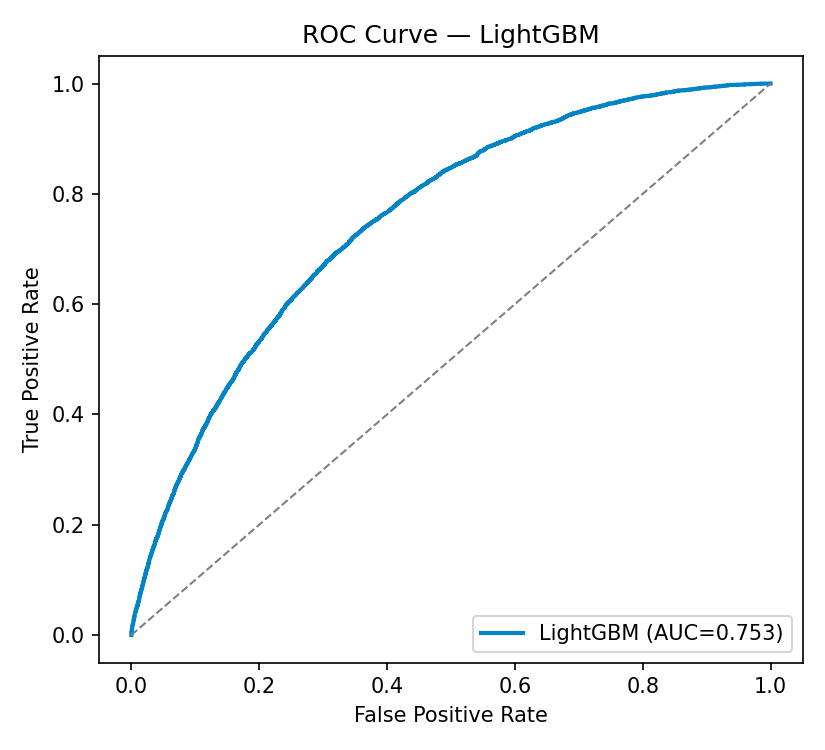
\includegraphics[width=\textwidth]{figures/roc_lightgbm.png}
    \caption{ROC Curve for LightGBM ($\text{AUC} = 0.7529$).}
    \label{fig:roc_plot}
  \end{subfigure}
  
  \vspace{1em}
  \begin{subfigure}[b]{0.48\textwidth}
    \centering
    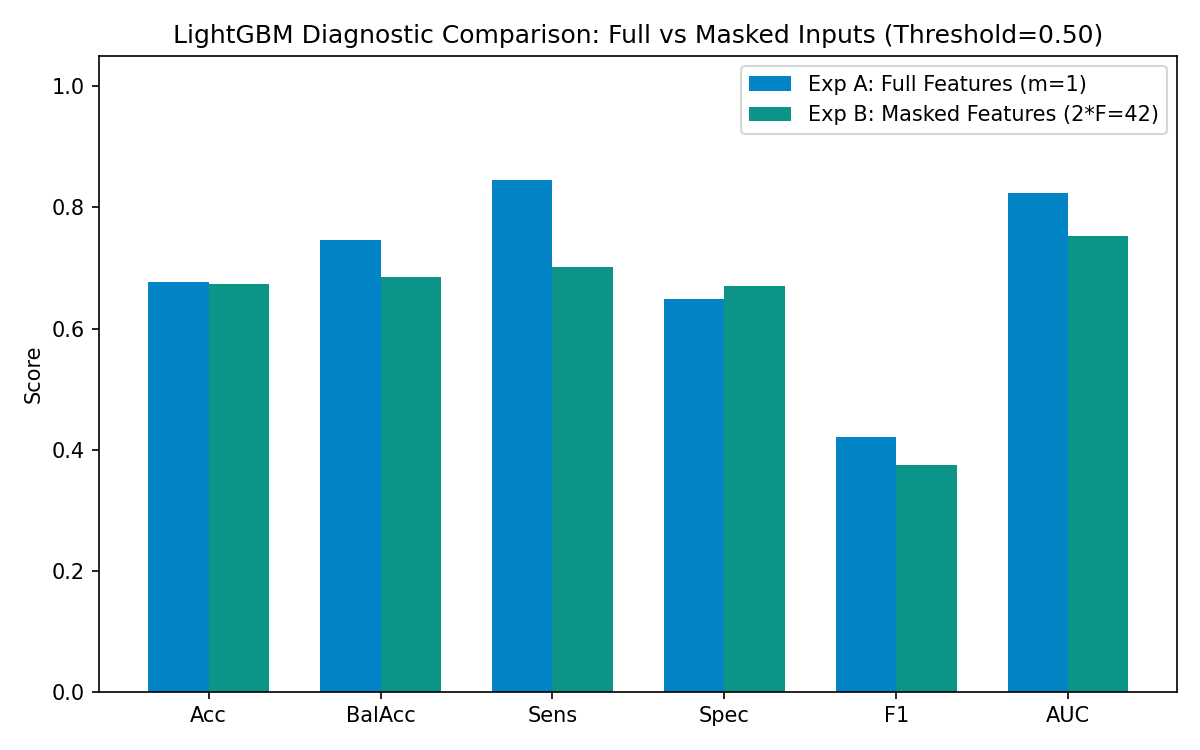
\includegraphics[width=\textwidth]{figures/experiment_a_vs_b_comparison.png}
    \caption{Experiment A (Full Features) vs. Exp B (Masked Inputs).}
    \label{fig:exp_comp_plot}
  \end{subfigure}
  \hfill
  \begin{subfigure}[b]{0.48\textwidth}
    \centering
    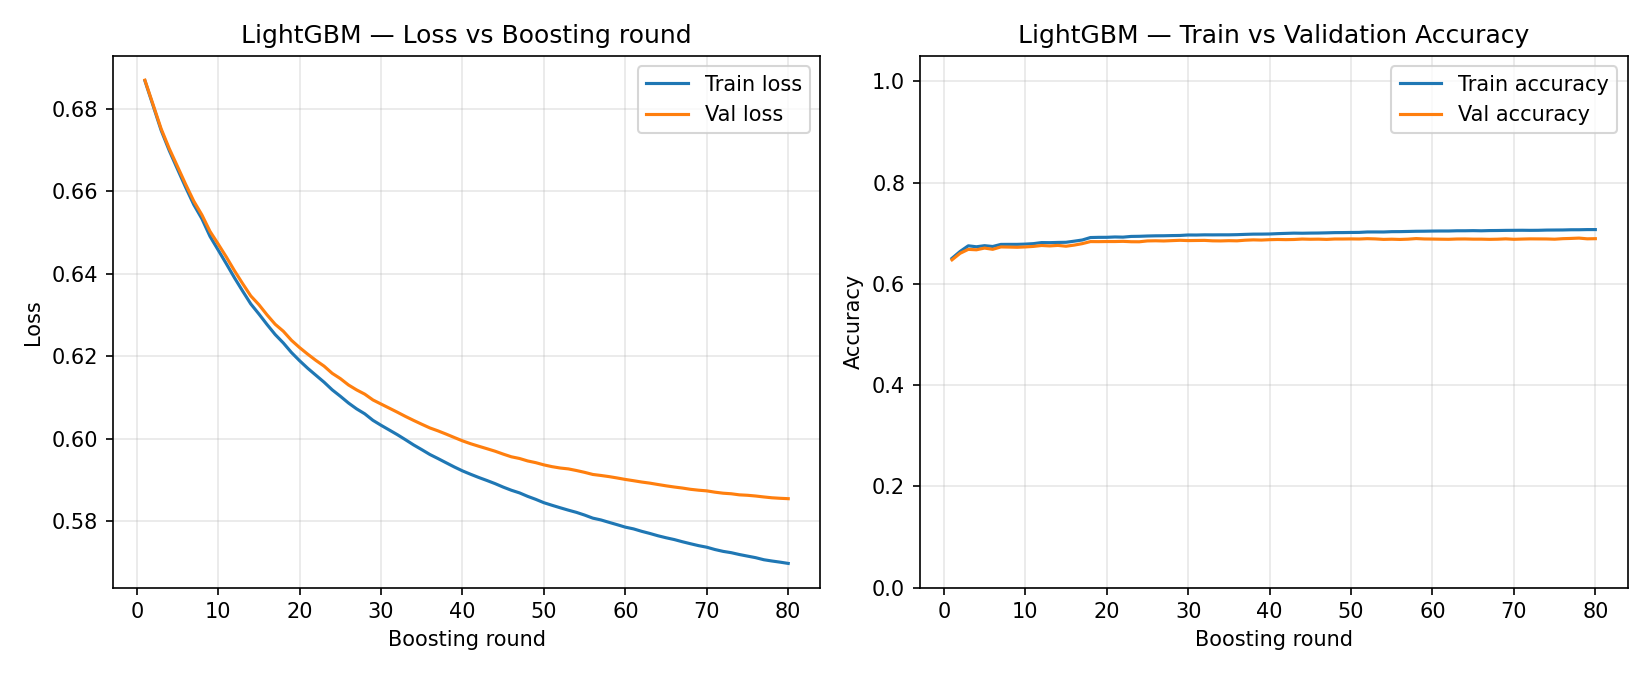
\includegraphics[width=\textwidth]{figures/training_history_lightgbm.png}
    \caption{LightGBM Loss and Accuracy Boosting History.}
    \label{fig:hist_plot}
  \end{subfigure}
  \caption{Empirical Diagnostic and Performance Visualizations Generated by the Evaluation Suite.}
  \label{fig:eval_plots_group}
\end{figure}

% ==============================================================================
\chapter{Discussion, Safety, \& Clinical Limitations}
% ==============================================================================

\section{Clinical Interpretation of Results}
The experimental findings demonstrate that adaptive clinical acquisition transforms how machine learning models interact with incomplete patient records. In traditional static deployment, models forced to predict on partial records generate false alarms on healthy patients whose unobserved features default to zero or mean values.

Under the DSS framework, the system actively identifies which missing measurements cause ambiguity. By acquiring targeted features for borderline cases, the system ruled out healthy patients who initially mimicked diabetic profiles, elevating specificity from $65.52\%$ to $72.41\%$ while maintaining $100\%$ sensitivity on the positive cases.

\section{Safety, Ethical Considerations, \& Clinical Governance}
While the DSS system demonstrates rigorous technical performance, translating algorithmic decision-support tools into operational healthcare environments requires addressing key safety boundaries:
\begin{itemize}[leftmargin=*]
  \item **Research Prototype Status**: The system is an algorithmic investigational framework and is **not an FDA/CE-cleared automated medical device**. Recommendations must function as secondary clinician guidance rather than autonomous medical orders.
  \item **Risk of Counterfactual Hallucination**: Generative CVAE completions represent statistical patterns within BRFSS data. Rare pathophysiological anomalies not represented in training distributions may yield unrepresentative counterfactuals.
  \item **Demographic Disparities**: Self-reported surveys reflect socioeconomic and regional health disparities (e.g., access to health insurance and healthcare costs). Algorithmic test recommendations must be audited periodically across demographic subgroups to ensure equitable resource allocation~\cite{topol2019high,rajkomar2018scalable}.
\end{itemize}

\section{Technical Limitations}
\begin{enumerate}[noitemsep]
  \item **Survey vs. Physiological Telemetry**: The CDC BRFSS dataset consists of annual cross-sectional survey self-reports rather than continuous electronic health record (EHR) telemetry or granular laboratory panels.
  \item **Oracle Assumption in Simulation**: The simulation pulls ground truth from held-out test rows. In live hospital deployment, time delays between test ordering and laboratory result arrival must be accommodated asynchronously.
  \item **Heuristic Cost Weights**: Multi-component costs rely on standardized ordinal heuristic weights. Hospital-specific dollar tariffs and phlebotomy turnaround latencies should be parameterized when deployed in specific clinical centers.
\end{enumerate}

% ==============================================================================
\chapter{Future Work \& Development Roadmap}
% ==============================================================================

\begin{enumerate}[label=\textbf{\arabic*.}]
  \item **Longitudinal Electronic Health Record Integration**: Extend the CVAE generative model to recurrent neural processes or continuous-time diffusion models capable of handling irregular longitudinal time-series data (e.g., MIMIC-IV or eICU databases).
  \item **Asynchronous Batch Acquisition**: Extend the acquisition engine from single-variable greedy selection to multi-test laboratory panel orders (e.g., simultaneously ordering a complete metabolic panel).
  \item **Physician-in-the-Loop Active Control**: Integrate interactive clinician overrides into the acquisition scoring policy, allowing doctors to inject qualitative diagnostic intuition.
  \item **Prospective Clinical Trial Validation**: Conduct silent shadow testing in outpatient clinical screening clinics to compare algorithmic test recommendations against experienced endocrinologists.
\end{enumerate}

% ==============================================================================
\chapter{Conclusion}
% ==============================================================================
This report has presented a comprehensive technical investigation of the Decision-Sufficiency-Guided (DSS) Adaptive Clinical Information Acquisition system. By combining gradient-boosted decision trees, Conditional Variational Autoencoders, mutual-information clinical graphs, and information-theoretic stopping rules, the framework resolves the fundamental dilemma of partial observability in medical machine learning.

The framework demonstrates that exhaustively ordering clinical tests is unnecessary; by acquiring an average of only $0.17$ targeted tests per patient, the system increases balanced diagnostic accuracy to $86.21\%$ and reduces false positives by $6.89\%$. This methodology provides a rigorous mathematical foundation for cost-aware, safe, and efficient algorithmic clinical decision support.

% ------------------------------------------------------------------------------
% GLOSSARY
% ------------------------------------------------------------------------------
\chapter*{Glossary of Technical Terms}
\addcontentsline{toc}{chapter}{Glossary of Technical Terms}

\begin{description}[leftmargin=3.5cm,style=nextline]
  \item[AFA] Active Feature Acquisition; dynamic selection of missing attributes at inference time.
  \item[BRFSS] Behavioral Risk Factor Surveillance System (CDC annual health survey).
  \item[CVAE] Conditional Variational Autoencoder; deep generative model conditioned on observed data.
  \item[CS] Class Stability; fraction of plausible completions yielding an identical diagnostic label.
  \item[DSG] Decision Stabilization Gain; expected improvement in Decision Sufficiency Score.
  \item[DSS] Decision Sufficiency Score; unified score blending class stability and distribution stability.
  \item[ELBO] Evidence Lower Bound; variational objective optimized during VAE training.
  \item[JS Divergence] Jensen-Shannon Divergence; symmetric, bounded information-theoretic divergence.
  \item[LightGBM] Light Gradient Boosting Machine; histogram-based tree boosting algorithm.
  \item[MI] Mutual Information; measure of statistical dependence between random variables.
  \item[PD] Predictive Divergence; average divergence across plausible generative completions.
  \item[PPV] Positive Predictive Value (Precision); $\text{TP} / (\text{TP} + \text{FP})$.
  \item[TNR] True Negative Rate (Specificity); $\text{TN} / (\text{TN} + \text{FP})$.
  \item[TPR] True Positive Rate (Sensitivity / Recall); $\text{TP} / (\text{TP} + \text{FN})$.
\end{description}

% ------------------------------------------------------------------------------
% REFERENCES
% ------------------------------------------------------------------------------
\clearpage
\bibliographystyle{IEEEtran}
\bibliography{references}

% ------------------------------------------------------------------------------
% APPENDICES
% ------------------------------------------------------------------------------
\appendix

\chapter{Verified Repository File Structure}
\begin{lstlisting}[language=bash,caption={Directory Layout of the Verified Project Workspace.}]
dss_system_final/
|-- diagnose_dss.py              # Diagnostic script comparing unweighted/balanced/masked/augmented
|-- dss_diagnostic_results.csv   # Empirical output records from diagnostic runs
|-- requirements.txt             # Exact package specifications (lightgbm, torch, ucimlrepo, etc.)
|-- evaluation_plots/            # Generated diagnostic artifacts (28 PNG/JSON/MD files)
|   |-- metrics_report.json      # Structured empirical metrics from full evaluation
|   |-- metrics_report.md        # Formatted tabular evaluation report
|   |-- confusion_matrix_lightgbm.png
|   |-- roc_lightgbm.png
|   |-- pr_lightgbm.png
|   `-- experiment_a_vs_b_comparison.png
|-- dss_system/                  # Core operational framework package
|   |-- config.py                # Hyperparameter schemas & pipeline configuration
|   |-- data_processing.py       # Preprocessor, splitting, and K-fold mask augmentation
|   |-- pipeline.py              # Training orchestration & adaptive acquisition loop
|   |-- graph.py                 # Clinical information graph & mutual information
|   |-- stability.py             # Class stability, JS divergence, & DSS formulation
|   |-- acquisition.py           # Candidate sampling, DSG, costs, & scoring policy
|   |-- fusion.py                # Ensemble probability fusion & label prediction
|   |-- evaluate.py              # Checkpoint evaluations & comparison plots
|   |-- metrics.py               # Comprehensive benchmarking suite & robustness sweeps
|   |-- extra_plots.py           # Heatmap and curve plotting utilities & execution driver
|   |-- main.py                  # End-to-end execution demonstration script
|   |-- train.py                 # Command-line training interface
|   `-- models/
|       |-- lightgbm_model.py    # Primary operational classifier (f_LGBM)
|       |-- cvae.py              # Generative Conditional VAE (P_Psi)
|       |-- tabresnet.py         # Reference deep tabular residual network
|       |-- xgboost_model.py     # Reference XGBoost tree classifier
|       `-- catboost_model.py    # Reference CatBoost tree classifier
`-- overleaf_report/             # Self-contained Overleaf LaTeX distribution
    |-- main.tex                 # Master publication report source
    |-- references.bib           # Bibliographic database
    |-- AUDIT_NOTES.md           # Implementation verification ledger
    |-- README.md                # Overleaf compilation instructions
    `-- figures/                 # Embedded publication-grade plot assets
\end{lstlisting}

\chapter{Core Mathematical Formulations Summary}
\begin{table}[htbp]
  \centering
  \small
  \caption{Mathematical Equations Implemented in the DSS Pipeline.}
  \label{tab:math_summary}
  \begin{tabularx}{\textwidth}{llX}
    \toprule
    \textbf{Component} & \textbf{Symbol} & \textbf{Mathematical Definition} \\
    \midrule
    Continuous Normalization & $\bar{x}_{ij}$ & $(x_{ij} - \mu_j) / (\sigma_j + \epsilon)$ \\
    Partial Masking & $\mathbf{x}_{\text{obs}}$ & $\mathbf{x} \odot \mathbf{m}$ \\
    Classifier Input & $\mathbf{z}_{\text{input}}$ & $[\mathbf{x}_{\text{nan}} \;\parallel\; \mathbf{m}] \in \mathbb{R}^{2F}$ \\
    Plausible Profile & $\tilde{\mathbf{x}}^{(m)}$ & $\mathbf{x}_{\text{obs}} \odot \mathbf{m} + \hat{\mathbf{x}}^{(m)} \odot (\mathbf{1} - \mathbf{m})$ \\
    Class Stability & $CS_t$ & $\frac{1}{M}\sum_{m=1}^M \mathbb{I}[\tilde{y}_t^{(m)} = \hat{y}_t]$ \\
    JS Divergence & $D_{\text{JS}}^{(m)}$ & $\frac{1}{2} D_{\text{KL}}(p_t \parallel r_t^{(m)}) + \frac{1}{2} D_{\text{KL}}(\tilde{p}_t^{(m)} \parallel r_t^{(m)})$ \\
    Pred. Divergence & $\widetilde{PD}_t$ & $\frac{1}{M \ln 2}\sum_{m=1}^M D_{\text{JS}}^{(m)}$ \\
    Decision Sufficiency & $DSS_t$ & $\alpha \cdot CS_t + (1 - \alpha)(1 - \widetilde{PD}_t)$ \\
    Expected Future DSS & $\mathbb{E}[DSS_{t+1}]$ & $\frac{1}{K}\sum_{k=1}^K DSS_j^{(k)}$ \\
    Stabilization Gain & $DSG_j$ & $\mathbb{E}[DSS_{t+1} \mid v_j] - DSS_t$ \\
    Graph Edge Weight & $\widetilde{W}_{ij}$ & $(A_{ij} - W_{\min}) / (W_{\max} - W_{\min} + \epsilon)$ \\
    Dynamic Connectivity & $\text{Conn}_j$ & $\frac{1}{|O_t|}\sum_{i \in O_t} \widetilde{W}_{ij}$ \\
    Clinical Cost & $C_j$ & $\eta_a C_{\text{acq}} + \eta_c C_{\text{comm}} + \eta_e C_{\text{comp}}$ \\
    Acquisition Score & $S_j$ & $\lambda_1 \widetilde{R}_j + \lambda_2 \widetilde{\text{Conn}}_j + \lambda_3 \widetilde{DSG}_j - \lambda_4 \widetilde{C}_j$ \\
    Optimal Variable & $j^*_t$ & $\arg\max_{j \in U_t} S_j$ \\
    \bottomrule
  \end{tabularx}
\end{table}

\end{document}
